%\section[A history of \shaone attacks]{The collision attack on \shaone from CRYPTO 2005, its ancestors and its developments}
\section{A brief history of collision attacks on \shaone}
\label{sec:history}

In this section we give a background on the literature of collision attacks on \shaone, that was initiated by the major work of Wang, Yin and Yu from CRYPTO~2005~\cite{DBLP:conf/crypto/WangYY05a}.
Some of the techniques used to attack \shaone had been previously introduced to attack other hash functions, and in particular \shazero, \shaone's close predecessor. Consequently, we start by
discussing some of these earlier work. We then review some of the more recent developments of the original attacks.

None of the material presented in this section is new, and it may be safely skipped by an experienced reader. We believe however that it may be of some use to a public less familiar with
the matter.

\medskip

All the attacks presented in this section are differential in nature. In its simplest form, the idea is to find a ``good'' \emph{message difference} $\diff(\expmess,\dexpmess)$
(or $\diff\expmess$)\footnote{Strictly speaking, the difference is imposed on the non-expanded message words $\mess_i$. However, the message expansion being linear,
we will usually rather consider the implied probability-one difference on the expanded message $\expmess_i$.}
and associated state differential path $\diff(\state,\dstate)$ (or $\diff\state$) such that: (1) A pair of states following the differential path
$\diff\state$ results in a collision; (2) Finding a pair of messages of difference $\diff\expmess$ such that the corresponding pair of states follows $\diff\state$ is
``efficient'' (in particular, this means that searching for a collision in that way is faster than searching for one by brute force).


\subsection{Preliminaries: collision attacks on \shazero}

In the initial SHA standard of 1993, there was no rotation by one to the left in the message expansion of the compression function~\cite{Nist-SHA0}; the corresponding original algorithm was
retrospectively named \shazero, to distinguish it from the updated standard \shaone, first published in 1995~\cite{Nist-SHA1}.
At CRYPTO~1998, Chabaud and Joux presented a theoretical collision attack on \shazero, with an estimated complexity of searching through $2^{61}$ message pairs~\cite{DBLP:conf/crypto/ChabaudJ98}
(equivalent to $2^{58}$ calls to the compression function of \shazero~\cite{DBLP:journals/joc/BihamCJ15}). However, the modified message
expansion of \shaone prevents a straightforward application of the same approach from leading to an attack better than brute force.

There are four main components in this original attack on \shazero (and its first improvements~\cite{DBLP:conf/crypto/BihamC04,DBLP:conf/eurocrypt/BihamCJCLJ05,DBLP:journals/joc/BihamCJ15}),
all of which found their way to the attacks on \shaone (either \emph{as is} or in a modified form):
\begin{enumerate}
\item \emph{Local collisions} in the step function as a springboard for a collision for the full function (\autoref{sec:local_coll}).
\item Using \emph{signed differences} and a fine analysis of difference conditions in the Boolean functions (\autoref{sec:diffs_ana}).
\item Regrouping local collisions along a \emph{disturbance vector} (\autoref{sec:dv_sha0}).
\item Efficient implementation of the probabilistic search for colliding messages (\autoref{sec:acc_techs_sha0}).
\end{enumerate}

We will only briefly mention the multi-block techniques as used for \shazero~\cite{DBLP:conf/eurocrypt/BihamCJCLJ05,DBLP:journals/joc/BihamCJ15}, as these are not directly relevant to the best attacks on \shaone.
The improvements by Wang \etal used to attack the full \shaone are presented next in \autoref{sec:full_sha1}.

\subsubsection{Local collisions for a few steps of \sha}
\label{sec:local_coll}
An instructive starting point when searching for collisions on \sha is to first consider a \emph{linearized} variant (over $\ftwo$) of the step function, obtained by replacing
the Boolean functions $\boolF_\text{IF}$ and $\boolF_\text{MAJ}$ by $\boolF_\text{XOR}$ and the additions in $\ztt$ by additions in $\ftwo^{32}$ (\ie XORs). Although collisions for this simple
variant (named \shiun by Chabaud and Joux~\cite{DBLP:conf/crypto/ChabaudJ98}) are trivial to find, \shiun is useful as a simple model to build the main structure of the attack
(in particular the differential paths $\diff\expmess$ and $\diff\state$),
one element of which being the concept of \emph{local collisions} for the step function.

It is easy to see (for instance from \autoref{eq:rec_step}) that only five consecutive state words are used in the step function of \sha to determine the value of the next (or previous) one. Consequently, if
we could introduce a difference in the message, such that after some steps the five current state words of $\state$ and $\dstate$ were equal, then the final hash values for the
two computations would form a collision,
as long as no more differences were present in the remainder of the message. Of course, the latter condition is hard to meet in general, but meeting the former seems to be quite easy as long as some limited
control on the message words is available. It is also a good first objective, as it locally achieves the result that we wish to get at the end of the computation.

\medskip

Let us assume that we have full control over six consecutive expanded message words: $\expmess_{i\ldots i + 5}$ and $\dexpmess_{i\ldots i + 5}$
used in the computation of two related \sha states $\state$, $\dstate$ and that we have $\expmess_j = \dexpmess_j$ for $j < i$.

The first step of a local collision is to introduce a difference (so that the two messages are not consistently equal, as we are not interested in any trivial equality),
for instance in one bit. For the linear variant \shiun, the exact index where this difference is introduced does not matter much;
let us assume w.l.o.g. that $\expmess_i$ and $\dexpmess_i$ are different exactly on bit 8, \ie
\begin{center}
\begin{tabular}{c}
$\diff(\expmess_i, \dexpmess_i) =$ \nodiff \nodiff \nodiff \nodiff \nodiff \nodiff \nodiff \nodiff \nodiff \nodiff \nodiff \nodiff \nodiff \nodiff
\nodiff \nodiff \nodiff \nodiff \nodiff \nodiff \nodiff \nodiff \nodiff \nodiff \onediff \nodiff \nodiff \nodiff \nodiff \nodiff \nodiff \nodiff \\
\end{tabular}.
\end{center}
From \autoref{eq:rec_step}, we see that this introduces a difference between $\state_{i + 1}$ and $\dstate_{i + 1}$ in the same position, \ie on bit 8. Our goal is now to ensure that this
difference does not propagate further, and that there is no difference between $\state_{i + 2\ldots i + 6}$ and $\dstate_{i + 2\ldots i + 6}$:
\begin{itemize}
\item At ($\state_{i + 2},\dstate_{i + 2}$), we must cancel the difference coming from $(\state_{(i + 2) - 1}, \dstate_{(i + 2) - 1}) \circlearrowleft 5 = (\state_{i + 1}, \dstate_{i + 1}) \circlearrowleft 5$;
this is done by inserting a difference in bit 13 of $\expmess_{i + 1}$:
\begin{center}
\begin{tabular}{c}
$\diff(\expmess_{i+1}, \dexpmess_{i+1}) =$ \nodiff \nodiff \nodiff \nodiff \nodiff \nodiff \nodiff \nodiff \nodiff
\nodiff \nodiff \nodiff \nodiff \nodiff \nodiff \nodiff \nodiff \nodiff \nodiff \onediff \nodiff \nodiff \nodiff \nodiff \nodiff \nodiff \nodiff \nodiff \nodiff \nodiff \nodiff \nodiff \\
\end{tabular}.
\end{center}
%
\item At ($\state_{i + 3},\dstate_{i + 3}$), we must cancel the difference coming from $(\state_{(i + 3) - 2}, \dstate_{(i + 3) - 2}) = (\state_{i + 1}, \dstate_{i + 1})$; this is done by inserting a difference in bit 8 of $\expmess_{i + 2}$:
\begin{center}
\begin{tabular}{c}
$\diff(\expmess_{i+2}, \dexpmess_{i+2}) =$ \nodiff \nodiff \nodiff \nodiff \nodiff \nodiff \nodiff \nodiff \nodiff \nodiff \nodiff \nodiff \nodiff \nodiff
\nodiff \nodiff \nodiff \nodiff \nodiff \nodiff \nodiff \nodiff \nodiff \nodiff \onediff \nodiff \nodiff \nodiff \nodiff \nodiff \nodiff \nodiff \\
\end{tabular}.
\end{center}
%
\item At ($\state_{i + 4},\dstate_{i + 4}$), we must cancel the difference coming from $(\state_{(i + 4) - 3}, \dstate_{(i + 4) - 3}) \circlearrowright 2 = (\state_{i + 1}, \dstate_{i + 1}) \circlearrowright 2$;
this is done by inserting a difference in bit 6 of $\expmess_{i + 3}$:
\begin{center}
\begin{tabular}{c}
$\diff(\expmess_{i+3}, \dexpmess_{i+3}) =$  \nodiff \nodiff \nodiff \nodiff \nodiff \nodiff \nodiff \nodiff \nodiff \nodiff \nodiff \nodiff \nodiff \nodiff \nodiff \nodiff
\nodiff \nodiff \nodiff \nodiff \nodiff \nodiff \nodiff \nodiff \nodiff \nodiff \onediff \nodiff \nodiff \nodiff \nodiff \nodiff\\
\end{tabular}.
\end{center}
%
\item At ($\state_{i + 5},\dstate_{i + 5}$), we must cancel the difference coming from $(\state_{(i + 5) - 4}, \dstate_{(i + 5) - 4}) \circlearrowright 2 = (\state_{i + 1}, \dstate_{i + 1}) \circlearrowright 2$;
this is done by inserting a difference in bit 6 of $\expmess_{i + 4}$:
\begin{center}
\begin{tabular}{c}
$\diff(\expmess_{i+4}, \dexpmess_{i+4}) =$  \nodiff \nodiff \nodiff \nodiff \nodiff \nodiff \nodiff \nodiff \nodiff \nodiff \nodiff \nodiff \nodiff \nodiff \nodiff \nodiff
\nodiff \nodiff \nodiff \nodiff \nodiff \nodiff \nodiff \nodiff \nodiff \nodiff \onediff \nodiff \nodiff \nodiff \nodiff \nodiff\\
\end{tabular}.
\end{center}
%
\item At ($\state_{i + 6},\dstate_{i + 6}$), we must cancel the difference coming from $(\state_{(i + 6) - 5}, \dstate_{(i + 6) - 5}) \circlearrowright 2 = (\state_{i + 1}, \dstate_{i + 1}) \circlearrowright 2$;
this is done by inserting a difference in bit 6 of $\expmess_{i + 5}$:
\begin{center}
\begin{tabular}{c}
$\diff(\expmess_{i+5}, \dexpmess_{i+5}) =$  \nodiff \nodiff \nodiff \nodiff \nodiff \nodiff \nodiff \nodiff \nodiff \nodiff \nodiff \nodiff \nodiff \nodiff \nodiff \nodiff
\nodiff \nodiff \nodiff \nodiff \nodiff \nodiff \nodiff \nodiff \nodiff \nodiff \onediff \nodiff \nodiff \nodiff \nodiff \nodiff\\
\end{tabular}.
\end{center}
\end{itemize}
At this point, we have reached our goal of having no differences in a pair of five consecutive state words.

The pattern formed by the successive message differences of a local collision is commonly seen in various stages of attacks on \sha, and as such it deserves to be shown in its entirety:
\begin{center}
\begin{tabular}{cc}
$\diff(\expmess_{i\ldots i+5}, \dexpmess_{i\ldots i+5}) =$ & \nodiff \nodiff \nodiff \nodiff \nodiff \nodiff \nodiff \nodiff \nodiff \nodiff \nodiff \nodiff \nodiff \nodiff
\nodiff \nodiff \nodiff \nodiff \nodiff \nodiff \nodiff \nodiff \nodiff \nodiff \onediff \nodiff \nodiff \nodiff \nodiff \nodiff \nodiff \nodiff \\
& \nodiff \nodiff \nodiff \nodiff \nodiff \nodiff \nodiff \nodiff \nodiff
\nodiff \nodiff \nodiff \nodiff \nodiff \nodiff \nodiff \nodiff \nodiff \nodiff \onediff \nodiff \nodiff \nodiff \nodiff \nodiff \nodiff \nodiff \nodiff \nodiff \nodiff \nodiff \nodiff \\
& \nodiff \nodiff \nodiff \nodiff \nodiff \nodiff \nodiff \nodiff \nodiff \nodiff \nodiff \nodiff \nodiff \nodiff
\nodiff \nodiff \nodiff \nodiff \nodiff \nodiff \nodiff \nodiff \nodiff \nodiff \onediff \nodiff \nodiff \nodiff \nodiff \nodiff \nodiff \nodiff \\
&  \nodiff \nodiff \nodiff \nodiff \nodiff \nodiff \nodiff \nodiff \nodiff \nodiff \nodiff \nodiff \nodiff \nodiff \nodiff \nodiff
\nodiff \nodiff \nodiff \nodiff \nodiff \nodiff \nodiff \nodiff \nodiff \nodiff \onediff \nodiff \nodiff \nodiff \nodiff \nodiff\\
&  \nodiff \nodiff \nodiff \nodiff \nodiff \nodiff \nodiff \nodiff \nodiff \nodiff \nodiff \nodiff \nodiff \nodiff \nodiff \nodiff
\nodiff \nodiff \nodiff \nodiff \nodiff \nodiff \nodiff \nodiff \nodiff \nodiff \onediff \nodiff \nodiff \nodiff \nodiff \nodiff\\
&  \nodiff \nodiff \nodiff \nodiff \nodiff \nodiff \nodiff \nodiff \nodiff \nodiff \nodiff \nodiff \nodiff \nodiff \nodiff \nodiff
\nodiff \nodiff \nodiff \nodiff \nodiff \nodiff \nodiff \nodiff \nodiff \nodiff \onediff \nodiff \nodiff \nodiff \nodiff \nodiff\\
\end{tabular}.
\end{center}

In the case of \shiun, the probability of obtaining a local collision when following the above pattern is equal to one. However, this is not the case anymore when the true \sha step function is used.
For instance, there is a probability $2^{-1}$ that the introduction of the difference in $(\state_{i+1},\dstate_{i+1})$ with modular addition rather than XOR
leads to a difference in more than one bit because of different
behaviours in the propagation of the carry in the two states (on which we do not assume to have any direct control). Overall, the probability of obtaining a successful local collision depends on several factors, including which Boolean function is used
and whether several collisions are chained together. We partially address this matter next.

\subsubsection{Difference analysis for impure ARX}
\label{sec:diffs_ana}
We now move away from \shiun and start to analyse the behaviour of local collisions for the true \sha function. There are two main points in this analysis: (1)~What conditions \emph{at the bit level}
ensure the highest probability of success for the different types of single local collisions; (2)~Under optimal conditions, what is the probability of a chain of interdependent local collisions?
We focus on the first question here, and defer the answer to the second to \autoref{sec:chain_lc}.

\medskip

In the case of \sha (and more generally ARX primitives), the way of expressing differences between messages is less obvious than for
\eg{} bit or byte-oriented primitives. It is indeed natural to consider both ``XOR differences'' (over $\ftwo^{32}$) and
``modular differences'' (over $\ztt$), as both operations are used in the function.
In practice, the literature on \sha uses several hybrid representations of differences based on \emph{signed XOR differences}.
In its most basic form, such a difference is similar to an XOR difference with the additional information of the value of the differing bits (and of bits equal to each other),
which is a ``sign'' for the difference.

This is an important information when one works with modular addition as the sign impacts the (absence of) propagation of carries in the addition of two differences.
Let us for instance consider the two pairs of words $a = 11011000001_b$, $\widetilde{a} = 11011000000_b$ and $b = 10100111000_b$, $\widetilde{b} = 10100111001_b$; the XOR
differences $(a \oplus \widetilde{a})$ and $(b \oplus \widetilde{b})$ are both $00000000001_b$ (\ie \nodiff\nodiff\nodiff\nodiff\nodiff\nodiff\nodiff\nodiff\nodiff\nodiff\onediff),
meaning that $(a \oplus b) = (\widetilde{a} \oplus \widetilde{b})$. On the other hand, the signed
XOR difference between $a$ and $\widetilde{a}$ may be written \nodiff\nodiff\nodiff\nodiff\nodiff\nodiff\nodiff\nodiff\nodiff\nodiff\onediffd to convey the fact that they are different on their lowest bit \emph{and} that
the value of this bit is 1 for $a$ (and thence 0 for $\widetilde{a}$), \ie $\widetilde{a} = a - 1$; similarly, the signed difference between $b$ and $\widetilde{b}$ may be written
\nodiff\nodiff\nodiff\nodiff\nodiff\nodiff\nodiff\nodiff\nodiff\nodiff\onediffu, which is a difference in the same position but of a different sign, \ie $\widetilde{b} = b + 1$. From these differences, we can deduce that $(a + b) = (\widetilde{a} + \widetilde{b})$
because differences of different signs cancel (while differences of the same sign do not); if we were to swap the values $b$ and $\widetilde{b}$, both differences on $a$ and $b$ would have the same sign and
indeed we have $(a + \widetilde{b}) \neq (\widetilde{a} + b)$ (though $(a \oplus \widetilde{b})$ and $(\widetilde{a} \oplus b)$ remain equal).
In the case of bits with no differences, we may similarly want to use different notations to express the fact that two bits are equal to zero (\nodiffz) or equal to one (\nodiffo).

It is possible to extend signed differences to account for more generic combinations of possible
values for each message bit; this was for instance done by De~Canni\`ere and Rechberger to aid in the automatic search of differential paths \cite{DBLP:conf/asiacrypt/CanniereR06}.
Another possible extension  is to consider relations between various bits of different (possibly rotated) state words;
this allows to efficiently keep track of the propagation of differences through the step function. Such differences are for instance used by Stevens \cite{DBLP:conf/eurocrypt/Stevens13},
and also later in this work.

\medskip

Using signed differences, we can express a first simple necessary condition for a local collision to happen: because the initial difference in $\diff\state_{i+1}$ has to be
canceled in $\diff\state_{i+2}$ through the modular addition of $\diff\expmess_{i+1}$, we know that these differences have to be of different sign. As we have some control on the
message, we can ensure that this is always the case for successful introductions of the difference on $\diff\state_{i+1}$ (that do not result in different carry propagations for
$\state_{i+1}$ and $\dstate_{i+1}$) by analysing what may happen in the four possible cases  of an introduction (depending on the signs of the involved differences), at the level of one bit:
\begin{enumerate}
\item \onediffu (the difference in $\diff\expmess_i$, introducing the perturbation) + \nodiffz (the ``difference'' in the same position of the partial sum used to compute $\diff\state_{i+1}$) = \onediffu,
with no different carry propagation in the remainder of $\diff\state_{i+1}$).
\item \onediffu  + \nodiffo = \onediffd, with different carry propagation.
\item \onediffd  + \nodiffz = \onediffd, with no different carry propagation.
\item \onediffd  + \nodiffo = \onediffu, with different carry propagation.
\end{enumerate}
Of these four cases, (1) and (3) are always favourable to a local collision; (2) and (4) are not considered to be favourable here, except if the differences are on the most significant bit
of the message and state words, as in this case the carry propagation is absorbed by the modular reduction (in that unique case, unsigned differences may be used safely)\footnote{We will
later see in \autoref{sec:chain_lc} that in some cases, a difference in the carry propagation does not actually always result in the absence of a local collision. We ignore this fact in the current analysis.}.
Thus, except when the difference is introduced on the MSB, we see that
a successful introduction on $\diff\state_{i+1}$ preserves the sign of the difference $\diff\expmess_i$, and thence we must always
choose a different sign for the difference on $\diff\expmess_{i+1}$ if we want the two to cancel.

We can analyse the rest of the conditions for a successful local collision in a similar fashion; it is helpful at this point to consider the possible behaviours of the Boolean functions of \sha
for their different signed inputs. We follow here the approach of Joux~\cite[Chapter 5]{algocrypt} and start by analysing the propagation of signed differences \nodiffz, \nodiffo,
\onediffd, \onediffu through $\boolF_\text{IF}$ (\autoref{tbl:diff_if}), $\boolF_\text{XOR}$ (\autoref{tbl:diff_xor}) and $\boolF_\text{MAJ}$ (\autoref{tbl:diff_xor}), before
considering what happens for each remaining correction of the local collision in $\diff\state_{i+3\ldots i+6}$.
An essentially identical analysis can for instance be found in~\cite{phdpeyrin,DBLP:journals/joc/BihamCJ15}.

We should note that for reasons that will be made clear in \autoref{sec:dv_sha0}, the corrections used to obtain a local collision must work with every possible Boolean function\footnote{This is not
true if our goal is to build boomerangs, which is something that we will consider in \autoref{sec:acc_techs_sha0}.}.
A consequence is that we cannot use the fact
that the non-linear functions $\boolF_\text{IF}$ and $\boolF_\text{MAJ}$ may absorb a single difference (as in \eg $\boolF_\text{IF}(\text{\nodiffz, \onediffu, \nodiffz})$),
as there is never such a behaviour with $\boolF_\text{XOR}$; thus, there is always a correction introduced in every message, true to the local collision pattern
of \shiun of \autoref{sec:local_coll}. In general, the following things may then happen in the Boolean functions: the difference is absorbed (this never happens
with $\boolF_\text{XOR}$);
the difference is preserved, but its sign is changed (this never happens with $\fmaj$); the difference is preserved and its sign is not changed.
As we already mentioned, knowing the sign of a difference is important if we want to cancel it with another one; thus, the possibility of
unpredictable changes of signs decreases the success probability of a local collision.
Let us see in general how this latter is impacted by the behaviours of the different Boolean functions.
\begin{itemize}
\item $\diff\state_{i+3}$: the difference is on the first input ($x$) of the Boolean function. With $\fif$, there is a probability $2^{-1}$ that it is absorbed and $2^{-2}$
that the sign is changed otherwise, for a total success probability of $2^{-2}$ ($2^{-1}$ on the MSB, where a change of sign has no consequence).
With $\fxor$, there is a probability $2^{-1}$ that the sign is changed (total success of $2^{-1}$, 1 on the MSB).
With $\fmaj$, there is a probability $2^{-1}$ that it is absorbed (total success of $2^{-1}$).
\item  $\diff\state_{i+4}$: the difference is on the second input ($y$) of the Boolean function. With $\fif$, there is a probability $2^{-1}$ that it is absorbed (total success of $2^{-1}$).
With $\fxor$ there is a probability $2^{-1}$ that the sign is changed (total success of $2^{-1}$, 1 on the MSB). With $\fmaj$ there is a probability $2^{-1}$ that it is absorbed (total success of
$2^{-1}$).
\item $\diff\state_{i+5}$: the difference is on the third input ($z$) of the Boolean function. This case is the same as for $\diff\state{i+4}$.
\item $\diff\state_{i+6}$: the difference is on a modular addition. If it is on the MSB, nothing needs to be done. Otherwise, it needs to be of sign opposite the one of the introductory difference to
ensure a correction (which will then happen with probability 1). This condition can be enforced for free by properly choosing the signed message difference $\diff\expmess$.
\end{itemize}

This analysis may be useful in several ways. First, it gives some necessary conditions on the signs of the corrections, possibly conditioned on the Boolean function of the round being considered;
more generally, it may actually be used as a (nearly) exhaustive list of inputs resulting in local collisions, but this is less useful as we do not have control on the values of $\diff\state$ in general. Second,
it helps us to position the local collisions in an ``optimal'' way, by ensuring that many corrections involve bits that are at the most significant position, as we have seen that these may
have higher success probabilities. Finally, it
may be used to check in advance if a given local collisions is going to happen or not, without necessarily computing the two states $\state$ and $\dstate$. For instance, in the first round,
assuming a perturbation on bit $j$ of $\diff\state_{i+1}$, we can predict that there will be no local collision if the bits $j - 2$ of $\diff\state_{i}$ and $\diff\state_{i-1}$ are equal, even if the perturbation is properly
introduced. Indeed, none of $\fif(\text{\onediffu,\nodiffz,\nodiffz})$, $\fif(\text{\onediffu,\nodiffo,\nodiffo})$, $\fif(\text{\onediffd,\nodiffz,\nodiffz})$, $\fif(\text{\onediffd,\nodiffo,\nodiffo})$
results in a difference
\footnote{This can also be trivially deduced from the very definition of the IF function.}, which means that there will be no difference in the Boolean function computation at $\diff\state_{i+3}$ and thus the tentative correction
in $\diff\expmess_{i+2}$ will actually introduce a difference.

\begin{table}[ht]
\caption{Signed difference analysis of $\boolF_\text{IF}(x,y,z)$.\label{tbl:diff_if}}
\begin{center}
\begin{tabularx}{\textwidth}{c | c c c c  X  c | c c c c}
\toprule
$x$ = \nodiffz & $y$ = \nodiffz & $y$ = \nodiffo & $y$ = \onediffu & $y$ = \onediffd & & $x$ = \nodiffo & $y$ = \nodiffz & $y$ = \nodiffo & $y$ = \onediffu & $y$ = \onediffd \\
\hline
$z$ = \nodiffz & \nodiffz & \nodiffz & \nodiffz & \nodiffz &                   & $z$ = \nodiffz & \nodiffz & \nodiffo & \onediffu & \onediffd\\
$z$ = \nodiffo & \nodiffo & \nodiffo & \nodiffo & \nodiffo &                   & $z$ = \nodiffo & \nodiffz & \nodiffo & \onediffu & \onediffd\\
$z$ = \onediffu & \onediffu & \onediffu & \onediffu & \onediffu &                   & $z$ = \onediffu & \nodiffz & \nodiffo & \onediffu & \onediffd\\
$z$ = \onediffd & \onediffd & \onediffd & \onediffd & \onediffd &                   & $z$ = \onediffd & \nodiffz & \nodiffo & \onediffu & \onediffd\\
\midrule
$x$ = \onediffu & $y$ = \nodiffz & $y$ = \nodiffo & $y$ = \onediffu & $y$ = \onediffd & & $x$ = \onediffd & $y$ = \nodiffz & $y$ = \nodiffo & $y$ = \onediffu & $y$ = \onediffd \\
\hline
$z$ = \nodiffz & \nodiffz & \onediffu & \onediffu & \nodiffz &                 & $z$ = \nodiffz & \nodiffz &  \onediffd & \nodiffz & \onediffd \\
$z$ = \nodiffo & \onediffd & \nodiffo & \nodiffo & \onediffd &                 & $z$ = \nodiffo & \onediffu & \nodiffo & \onediffu & \nodiffo \\
$z$ = \onediffu & \nodiffz & \onediffu & \onediffu & \nodiffz &                & $z$ = \onediffu & \onediffu & \nodiffo & \onediffu & \nodiffo \\
$z$ = \onediffd & \onediffd & \nodiffo & \nodiffo & \onediffd &                & $z$ = \onediffd & \nodiffz & \onediffd & \nodiffz & \onediffd\\
\bottomrule
\end{tabularx}
\end{center}
\end{table}

\begin{table}[ht]
\caption{Signed difference analysis of $\boolF_\text{XOR}(x,y,z)$.\label{tbl:diff_xor}}
\begin{center}
\begin{tabularx}{\textwidth}{c | c c c c  X  c | c c c c}
\toprule
$x$ = \nodiffz & $y$ = \nodiffz & $y$ = \nodiffo & $y$ = \onediffu & $y$ = \onediffd & & $x$ = \nodiffo & $y$ = \nodiffz & $y$ = \nodiffo & $y$ = \onediffu & $y$ = \onediffd \\
\hline
$z$ = \nodiffz & \nodiffz & \nodiffo & \onediffu & \onediffd &                   & $z$ = \nodiffz & \nodiffo & \nodiffz & \onediffd & \onediffu\\
$z$ = \nodiffo & \nodiffo & \nodiffz & \onediffu & \onediffd &                   & $z$ = \nodiffo & \nodiffz & \nodiffo & \onediffd & \onediffu\\
$z$ = \onediffu & \onediffu & \onediffd & \nodiffz & \nodiffo &                   & $z$ = \onediffu & \onediffd & \onediffu & \nodiffo & \nodiffz\\
$z$ = \onediffd & \onediffd & \onediffu & \nodiffo & \nodiffz &                   & $z$ = \onediffd & \onediffu & \onediffd & \nodiffz & \nodiffo\\
\midrule
$x$ = \onediffu & $y$ = \nodiffz & $y$ = \nodiffo & $y$ = \onediffu & $y$ = \onediffd & & $x$ = \onediffd & $y$ = \nodiffz & $y$ = \nodiffo & $y$ = \onediffu & $y$ = \onediffd \\
\hline
$z$ = \nodiffz & \onediffu & \onediffd & \nodiffz & \nodiffo &                 & $z$ = \nodiffz & \onediffd &  \onediffu & \nodiffo & \nodiffz \\
$z$ = \nodiffo & \onediffd & \onediffu & \nodiffo & \nodiffz &                 & $z$ = \nodiffo & \onediffu & \onediffd & \nodiffz & \nodiffo \\
$z$ = \onediffu & \nodiffz & \nodiffo & \onediffu & \onediffd &                & $z$ = \onediffu & \nodiffo & \nodiffz & \onediffd & \onediffu \\
$z$ = \onediffd & \nodiffo & \nodiffz & \onediffd & \onediffu &                & $z$ = \onediffd & \nodiffz & \nodiffo & \onediffu & \onediffd\\
\bottomrule
\end{tabularx}
\end{center}
\end{table}

\begin{table}[ht]
\caption{Signed difference analysis of $\boolF_\text{MAJ}(x,y,z)$.\label{tbl:diff_maj}}
\begin{center}
\begin{tabularx}{\textwidth}{c | c c c c  X  c | c c c c}
\toprule
$x$ = \nodiffz & $y$ = \nodiffz & $y$ = \nodiffo & $y$ = \onediffu & $y$ = \onediffd & & $x$ = \nodiffo & $y$ = \nodiffz & $y$ = \nodiffo & $y$ = \onediffu & $y$ = \onediffd \\
\hline
$z$ = \nodiffz & \nodiffz & \nodiffz & \nodiffz & \nodiffz &                   & $z$ = \nodiffz & \nodiffz & \nodiffo & \onediffu & \onediffd\\
$z$ = \nodiffo & \nodiffz & \nodiffo & \onediffu & \onediffd &                   & $z$ = \nodiffo & \nodiffo & \nodiffo & \nodiffo & \nodiffo\\
$z$ = \onediffu & \nodiffz & \onediffu & \onediffu & \nodiffz &                   & $z$ = \onediffu & \onediffu & \nodiffo & \onediffu & \nodiffo\\
$z$ = \onediffd & \nodiffz & \onediffd & \nodiffz & \onediffd &                   & $z$ = \onediffd & \onediffd & \nodiffo & \nodiffo & \onediffd\\
\midrule
$x$ = \onediffu & $y$ = \nodiffz & $y$ = \nodiffo & $y$ = \onediffu & $y$ = \onediffd & & $x$ = \onediffd & $y$ = \nodiffz & $y$ = \nodiffo & $y$ = \onediffu & $y$ = \onediffd \\
\hline
$z$ = \nodiffz & \nodiffz & \onediffu & \onediffu & \nodiffz &                 & $z$ = \nodiffz & \nodiffz &  \onediffd & \nodiffz & \onediffd \\
$z$ = \nodiffo & \onediffu & \nodiffo & \onediffu & \nodiffo &                 & $z$ = \nodiffo & \onediffd & \nodiffo & \nodiffo & \onediffd \\
$z$ = \onediffu & \onediffu & \onediffu & \onediffu & \onediffu &                & $z$ = \onediffu & \nodiffz & \nodiffo & \onediffu & \onediffd \\
$z$ = \onediffd & \nodiffz & \nodiffo & \onediffu & \onediffd &                & $z$ = \onediffd & \onediffd & \onediffd & \onediffd & \onediffd\\
\bottomrule
\end{tabularx}
\end{center}
\end{table}

% two things: 1) optimal conditions; 2) proba (w. interactions) given optimal conditions

\subsubsection{Disturbance vectors}
\label{sec:dv_sha0}

We have seen how using a local collision allows one to create a pair of different messages which may lead to a pair of \sha states that are identical at some point during the
computation of their respective digests. Given enough control on the message (which implies control on the state), one may obtain such an equality with probability one, and it is quite easy to derive sufficient conditions
for a single local collision to happen, which allows to derive the success probability of uncontrolled independent local collisions.

In order to mount a complete attack and obtain a collision on the actual digest, we need to ensure that the last five state words are free of differences: this means that no local collision
must have been started after step 75. Of course, we also need the colliding messages to be valid expanded messages, and this is where local collisions become really useful: the idea is to
interleave a series of local collisions together so that: (1)~The resulting message difference follows the message expansion; (2)~The joint probability of all the local collisions being successful
is high (in particular, an attack is obtained if it is higher than $\approx 2^{-80}$).

The first condition is actually easy to meet by defining a \emph{disturbance vector} (\dv). This is a vector of eighty 32-bit words, with its `1' bits defining the positions of the initial perturbations of the series
of local collisions.
Now it suffices to remark that because the message expansion is linear, a sum of expanded messages is an expanded message itself;
then if the disturbance vector is a valid expanded message word, so is the complete message difference, including the corrections of the local
collisions. For this to be correct, however, two conditions need to be met: (1)~The disturbance vector must have no differences in its first five ``negative'' words $\expmess_{-5,\ldots,-1}$, obtained through
the backward message expansion. Indeed, remembering \autoref{sec:local_coll}, the corrections of the local collisions will be obtained from (possibly rotated) shifted copies of the pattern of initial perturbations introduced by the \dv,
up to five positions down. If we want these copies to be valid expanded message words, they must be equal to the \dv with its last (up to five) words removed and with a few (up to five) words
added at the beginning, which would be obtained from the backward message expansion. As the added words must be zero, lest they create new perturbations that would not be corrected, we obtain the aforementioned
condition. (2)~All corrections need to be performed in the same way, so that they globally conform to the message expansion; this is why one cannot exploit the absorption properties of some Boolean functions as noticed in \autoref{sec:diffs_ana},
as it is impossible to do so consistently across all the rounds.

This simple characterization of series of local collisions allows to define efficient search strategies to find vectors
that achieve a high joint probability.
In the case of \shazero, the message expansion can easily be defined at the bit level, as the bit $i$ of an expanded message word $\expmess_j$, $j > 15$ is entirely determined by the bit $i$
of the message words $\expmess_{j-16\ldots j-1}$. This means that any expanded message (and in particular a disturbance vector) can be seen as the union of 32 ``one-bit expanded messages'' that
do not interact with each other. Thus, a search for good disturbance vectors can focus solely on such one-bit messages. As any consecutive window of sixteen message words entirely
defines the remainder of an expanded message word through the (backward) message expansion, one can see that there is only a small number of $2^{16}$ one-bit disturbance vectors to consider, which
can then be shifted laterally to start on any of the 32 bits of a message word.

Of the $2^{16}$ candidate disturbance vectors, many do not meet the condition of being zero on their first five negative positions and their last five positions. Overall, these requirements give
``10 bits of conditions'', and indeed only $2^6$ vectors meet all of them (one of them being the all-zero vector)~\cite[Chapter 5]{algocrypt}. It now remains to determine which of these lead
to the best attacks.

\medskip

A first (rather crude) way of estimating the cost of a collision associated with a certain \dv is simply to count the number of local collisions it introduces (\ie to consider the Hamming weight
of the vector) and to multiply this by the probability of a local collision being successful. This estimate can immediately be enhanced by discounting the cost of collisions appearing in the
first sixteen state words, as the attacker has a full control on the corresponding message words and can then fulfill all their associated conditions deterministically. Additionally, recalling
\autoref{sec:diffs_ana}, we know that the success probability of a local collision increases if some of the bit differences are located on the MSB. Thus, the probability of a \dv is not
invariant by lateral shift, and each vector should be considered on its best positions only (given the pattern of corrections of a local collision, inserting the perturbations on
bit one (starting from zero) is a good choice).

There is one problem remaining with this first cost function, which is that it assumes that all local collisions are independent. This is actually not the case, and a more detailed analysis of
the success probability of non-independent local collisions is necessary to get an accurate estimate of the overall cost of an attack. We do not detail such an analysis in the present case
of \shazero, and instead refer to \cite[Chapter 5]{algocrypt}, which shows possible interactions between local collisions in a case-by-case study. The main result of this is that
some interactions introduce contradictions that cannot be resolved and which thence entirely disqualify some \dvs (this may happen in particular because of the absorption capabilities
of $\boolF_\text{IF}$; in that case, it disqualifies \dvs with two consecutive perturbations in the first round (the ``IF'' round)),
while the probability of some other interactions being successful can be increased by properly choosing the sign of some specific collisions. We will later discuss
the issue further for \shaone in \autoref{sec:chain_lc}.

With this refined cost function in mind, two good disturbance vectors where found for the original attack on \shazero~\cite{DBLP:conf/crypto/ChabaudJ98}; we show the first of them in
\autoref{fig:shaz_dv}, using an unsigned differences notation.

\begin{figure}[ht]
\begin{center}
\nodiff \nodiff \nodiff \onediff \nodiff \nodiff \nodiff \nodiff \nodiff \nodiff \nodiff \onediff \nodiff \nodiff \onediff \nodiff \nodiff \nodiff \nodiff \nodiff
\nodiff \nodiff \onediff \nodiff \nodiff \nodiff \nodiff \onediff \onediff \nodiff \onediff \onediff \nodiff \onediff \onediff \onediff \onediff \onediff \onediff \nodiff\\

\onediff \onediff \nodiff \onediff \nodiff \nodiff \onediff \nodiff \nodiff \nodiff \nodiff \onediff \nodiff \onediff \nodiff \onediff \nodiff \nodiff \onediff \nodiff
\onediff \nodiff \onediff \nodiff \nodiff \nodiff \onediff \nodiff \onediff \onediff \onediff \nodiff \nodiff \onediff \onediff \nodiff \nodiff \nodiff \nodiff \nodiff
\end{center}
\caption[A good (one bit) disturbance vector for \shazero.]{A good (one bit) disturbance vector for \shazero, with a basic cost of $2^{68}$. Bit zero is shown on the top left.\label{fig:shaz_dv}}
\end{figure}

\subsubsection{Accelerating techniques for collision search}
\label{sec:acc_techs_sha0}

A suitable disturbance vector such as the one of \autoref{fig:shaz_dv} defines an explicit attack procedure in a straightforward way: one uses the available freedom in the first
sixteen message words to deterministically fulfill as many conditions for local collisions, while keeping enough free bits to expect being able to fulfill the remaining conditions
probabilistically.

This was the approach taken in the original attack on \shazero, and it results in an attack of complexity $2^{67}$ (measured in the number of message pairs to be tested for a collision)
for the vector of \autoref{fig:shaz_dv}, and $2^{61}$ for another good disturbance vector~\cite{DBLP:conf/crypto/ChabaudJ98}.

Although this is already an attack that is significantly faster than a brute-force approach, it remains fairly expensive, and no explicit collision for \shazero was computed at the time\footnote{Even
nearly twenty years later, such an attack requires considerable resources; it would roughly be comparable in cost with the full free-start collision for \shaone which is the main topic of
this part.}.
A series of techniques were later developed to make such attacks considerably more efficient, which ultimately led to the first explicit collision on \shazero~\cite{DBLP:conf/eurocrypt/BihamCJCLJ05}.
These improvements were of two kinds: (1) Chaining multiple blocks to enable the use of better \dvs; (2) Using \emph{neutral bits} to make the probabilistic phase of the attack more efficient.
The first improvement as originally used for \shazero was later superseded by the two-block attack structure of Wang \etal, used both for improved attacks on \shazero
and for the first full theoretical attack on \shaone~\cite{DBLP:conf/crypto/WangYY05,DBLP:conf/crypto/WangYY05a},
and we will not describe it here. The second improvement,
originally introduced by Biham and Chen~\cite{DBLP:conf/crypto/BihamC04} was much more long-lived, and it is still useful in current attacks, including ours.

The aim of the neutral bits technique is to make a better use of the available freedom in the first sixteen message words, in order to speed up the attack. The idea is to identify bits
of messages that with good probability do not interact with any local collision necessary conditions, say up to step $n$. Thus, if one found a message pair fulfilling all conditions
up to step $n$ (a \emph{partial solution}), flipping a neutral bit will lead to another message pair similarly fulfilling all conditions up to $n$ with good probability. Using neutral bits then allows to amortize
the cost of finding good message pairs, which makes the attack faster. To make things a bit more formal, we may give the following:

\begin{defi}[Neutral bits]
A bit $b$ of $\expmess_{0 \leq i < 16}$ is a \emph{neutral bit} for a disturbance vector $\mathcal{V}$ at step $n$ with probability $p$ if the probability (taken over the message space) that it does not interact
with any necessary condition for $\mathcal{V}$ up to step $n$ is equal to $p$.
\end{defi}

This definition can be generalized by considering groups of bits that need to be flipped together. This may be done either because it makes these bits being more effective, or because not doing so would
change the sign of some bits of local collisions later in the expanded message.

In general, one can distinguish two (not mutually excluding) approaches to finding neutral bits: either running a random search across many partial solutions; or using the propagation properties of the step function to identify
good candidates. In particular, the latter approach found a powerful expression with the technique of auxiliary differential paths (or \emph{boomerangs}), first developed for \shaone~\cite{DBLP:conf/crypto/JouxP07}
and which led to the currently fastest attacks on \shazero~\cite{DBLP:conf/fse/ManuelP08}.

A boomerang in that context is a small set of neutral bits that are particularly efficient when activated together (\ie of the first kind mentioned above), in particular because they define a local collision (or possibly
a few of them) for which all necessary conditions have been pre-satisfied. Flipping the bits of the boomerang then only introduces a single local perturbation that is immediately corrected and thus does not propagate.
Yet, because the local collision defined by the neutral bits is not chained along a disturbance vector, uncorrected perturbations will eventually be introduced by the message expansion and result in interactions
with necessary conditions; this will however happen much later than with ``standard'' neutral bits. One can notice that because the local collisions of a boomerang do not need to be chained, they do not need to
be of a form suitable for every Boolean function. For instance, as it was hinted earlier in \autoref{sec:diffs_ana}, one can obtain better boomerangs by using the absorption properties of the IF function to define
local collisions with fewer necessary corrections.

We conclude this short summary on \shazero by giving an illustration of the different phases of a one-block attack on \shazero in \autoref{fig:struct_shazero}. The two main rectangles represent the state and
expanded messages of a computation of \shazero. The diagonal lines (\,\begin{tikzpicture}[scale=0.25]\draw[thick,pattern=north west lines] (0,0) rectangle (1,1);\end{tikzpicture}\,,
\begin{tikzpicture}[scale=0.25]\draw[thick,pattern=north east lines] (0,0) rectangle (1,1);\end{tikzpicture}\,) represent areas of the state and messages that are fixed for an attack; any state condition within this zone is deterministically fulfilled.
The non-diagonal lines in the message represent bits that are used to generate many message pairs in the hope that one leads to a collision; horizontal lines
(\,\begin{tikzpicture}[scale=0.25]\draw[thick,pattern=horizontal lines] (0,0) rectangle (1,1);\end{tikzpicture}\,) do so purely probabilistically, and vertical lines
(\,\begin{tikzpicture}[scale=0.25]\draw[thick,pattern=vertical lines] (0,0) rectangle (1,1);\end{tikzpicture}\,)
represent neutral bits which are useful to amortize the cost of finding partial solutions; the (completely determined) remainder of the expanded message is left blank.
Finally, dots
(\,\begin{tikzpicture}[scale=0.25]\draw[thick,pattern=dots] (-1,-1) rectangle (0,0);\end{tikzpicture}\,)
represent conditions that need to be fulfilled probabilistically.
%; denser zones indicate a higher probability
%of satisfying all conditions within.

\begin{figure}[!htb]
\begin{center}
% defining the new dimensions
\newlength{\starsize}
\newlength{\starspread}
% declaring the keys in tikz
\tikzset{starsize/.code={\setlength{\starsize}{#1}},
         starspread/.code={\setlength{\starspread}{#1}}}
% setting the default values
\tikzset{starsize=1mm,
         starspread=3mm}
% declaring the pattern
\pgfdeclarepatternformonly[\starspread,\starsize]% variables
  {custom fivepointed stars}% name
  {\pgfpointorigin}% lower left corner
  {\pgfqpoint{\starspread}{\starspread}}% upper right corner
  {\pgfqpoint{\starspread}{\starspread}}% tilesize
  {% shape description
   \pgftransformshift{\pgfqpoint{\starsize}{\starsize}}
   \pgfpathmoveto{\pgfqpointpolar{18}{\starsize}}
   \pgfpathlineto{\pgfqpointpolar{162}{\starsize}}
   \pgfpathlineto{\pgfqpointpolar{306}{\starsize}}
   \pgfpathlineto{\pgfqpointpolar{90}{\starsize}}
   \pgfpathlineto{\pgfqpointpolar{234}{\starsize}}
   \pgfpathclose%
   \pgfusepath{fill}
  }



\begin{tikzpicture}[scale=0.22,>=latex']
%\begin{tikzpicture}[scale=0.17,>=latex']
    % teh boxez
    \draw[thick] (0,0) -- (20,0) -- (20,-34);
    \draw[thick,dashed] (20,-34) -- (15,-33) -- (10,-34) -- (5,-33) -- (0,-34);
    \draw[thick] (0,-34) -- (0,0);
    \draw[thick] (25,-4) -- (45,-4) -- (45,-34);
    \draw[thick,dashed] (45,-34) -- (40,-33) -- (35,-34) -- (30,-33) -- (25,-34);
    \draw[thick] (25,-34) -- (25,-4);
    % teh row indices for the state
    \node at (-2,0) {-4};
    \node at (-2,-4) {0};
    \node at (-2,-20) {16};
    \node at (-2,-26) {22};
    \node at (-2,-34) {30};
    % teh row indices for the message
    \node at (23,-4) {0};
    \node at (23,-19) {15};
    % the fillings
    \draw[pattern=crosshatch] (0,0) rectangle (20,-4); % IV
    \fill[pattern=north west lines] (0,-4) rectangle (20,-18); % base solution
    \fill[pattern=north west lines] (0,-18) -- (7,-18) -- (0,-22); % base solution
    \fill[pattern=north west lines] (13,-18) -- (20,-18) -- (20,-22); % base solution
	\draw (0,-22) -- (7,-18) -- (13,-18) -- (20,-22);
    \fill[pattern=custom fivepointed stars,starspread=1.4mm,starsize=0.5mm] (0,-22.2) -- (7,-18) -- (13,-18) -- (20,-22.2); % NB 1
	\fill[pattern=custom fivepointed stars,starspread=1.7mm,starsize=0.5mm] (0,-22.4) rectangle (20,-26); % NB 2
    \fill[pattern=custom fivepointed stars,starspread=2.1mm,starsize=0.5mm] (0,-26.1) rectangle (20,-30); % NB 3
    \fill[pattern=custom fivepointed stars,starspread=2.5mm,starsize=0.5mm] (0,-30) rectangle (20,-33); % NB 6
	\fill[pattern=north east lines] (25,-4) rectangle (45,-15); % message
	\fill[pattern=north east lines] (25,-15) --  (32,-15) -- (29,-19) -- (25,-19) ; % message
	\fill[pattern=north east lines] (38,-15) --  (45,-15) -- (45,-19) -- (41,-19) ; % message
	\draw (25,-19) -- (29,-19) --  (32,-15) -- (38,-15) -- (41,-19) -- (45,-19);
	\draw (25,-19) -- (41,-19);
	\fill[pattern=vertical lines] (32,-15) -- (38,-15) -- (41,-19);
	\fill[pattern=horizontal lines] (29,-19) -- (32,-15) -- (41,-19);

    % legends
    \draw[thick] (50,-8) rectangle (51.5,-9.5);
    \node[anchor=text] at (55,-9.5) {$\iv$};
    \draw[pattern=crosshatch] (50,-8) rectangle (51.5,-9.5);
    %
    \draw[thick] (50,-12) rectangle (51.5,-13.5);
    \node[anchor=text] at (55,-13.5) {Deterministic};
    \node[anchor=text] at (55,-15) {conditions};
    \draw[pattern=north west lines] (50,-12) rectangle (51.5,-13.5);
    %
    \draw[thick] (50,-16) rectangle (51.5,-17.5);
    \node[anchor=text] at (55,-17.5) {Probabilistic};
    \node[anchor=text] at (55,-19) {conditions};
    \draw[pattern=custom fivepointed stars,starspread=1.2mm,starsize=0.5mm] (50,-16) rectangle (51.5,-17.5);
    %
    \draw[thick] (50,-20) rectangle (51.5,-21.5);
    \node[anchor=text] at (55,-21.5) {Fixed};
    \node[anchor=text] at (55,-23) {message};
    \draw[pattern=north east lines] (50,-20) rectangle (51.5,-21.5);
    %
    \draw[thick] (50,-24) rectangle (51.5,-25.5);
    \node[anchor=text] at (55,-25.5) {Randomized};
    \node[anchor=text] at (55,-27) {message};
    \draw[pattern=horizontal lines] (50,-24) rectangle (51.5,-25.5);
    %
    \draw[thick] (50,-28) rectangle (51.5,-29.5);
    \node[anchor=text] at (55,-29.5) {Neutral bits};
    \draw[pattern=vertical lines] (50,-28) rectangle (51.5,-29.5);

    %title
    \node[anchor=text] at (0,3) {\shazero State words ($\state_i$)};
    \node[anchor=text] at (25,3) {\shazero Message words ($\expmess_i$)};

\end{tikzpicture}

\end{center}
\caption{The structure of a one-block attack on \shazero.\label{fig:struct_shazero}}
\end{figure}

\subsection{Collision attacks on the full \shaone}
\label{sec:full_sha1}

Having discussed the original attacks on \shazero, we now turn our attention to \shaone for the rest of this chapter. Although both functions are very similar, their different message expansion makes a direct
application of attacks on \shazero in the form discussed above inapplicable to the full \shaone. We now discuss the new techniques that were developed for that purpose and some of their
subsequent improvements:
\begin{enumerate}
\item The use of \emph{non-linear} differential paths and of a two-block attack structure is the main improvement that makes full attacks on \shaone possible (\autoref{sec:nl_struct}).
\item The different message expansion of \shaone makes the search for good disturbance vectors more complex (\autoref{sec:sha1_dvs}).
\item Better cost functions were defined for the disturbance vectors (\autoref{sec:chain_lc}).
\end{enumerate}
It is important to note that although these improvements were somehow necessary to attack \shaone and led to the first theoretical attack on this function~\cite{DBLP:conf/crypto/WangYY05a},
the same technique can, and were, applied to improve the existing attacks on \shazero as well~\cite{DBLP:conf/crypto/WangYY05}, and also other functions of the \mdsha family.

Let us also mention for completeness that the original attacks of Wang \etal used an accelerating technique named \emph{message modification} instead of neutral bits. Such a technique works
by identifying changes in message words controlled by the attacker that only impact (say) a single necessary condition for a local collision located at a point where no direct control is possible.
This can be used during the probabilistic phase of the attack to carefully fulfill some of the conditions independently of each other, which increases the probability of success. However, it is not
clear whether this technique has a significant advantage over neutral bits (especially when including boomerangs), and it is somehow harder to implement efficiently, especially on a parallel architecture. Thus, we will not detail it
further in this chapter.

\subsubsection{The two-block structure and non-linear paths}
\label{sec:nl_struct}
% incl. automated search
With the benefit of hindsight, looking back on the case of \shazero, we can identify two points in particular where the original attack does not seem to be optimal:
\begin{enumerate}
\item The original structure with a single block imposes the \dv to be zero in its last five bits, which may disqualify some otherwise good
\dvs. A way to get around this restriction is to use ``multi-block'' attacks (which culminated in using only two blocks).
\item Using a purely linearized model for the propagation of differences in the round function similarly imposes the condition that the first
five negative bits of the \dv have to be zero, and that there are no consecutive bits during the IF round. A way to remove these conditions
is to switch to a non-linear propagation model for (part of) the first round.
\end{enumerate}
We now discuss these two improvements in more detail.

\paragraph{The two-block structure.}
In a multi-block attack, one uses \dvs which only result in \emph{near collisions},
\ie final states still containing a few differences, only in controlled locations. The idea is then to chain such \dvs together in a way
that eventually produces a collision, by cancelling in the last block the few differences in the \iv (coming from a near collision in the previous block
through the Merkle-Damg\aa rd domain extension) with appropriate differences in the final state, thanks to the feed-forward of the
Davies-Meyer construction.

This was first done by Biham \etal to obtain the first explicit collision on \shazero, using four blocks of different
\dvs~\cite{DBLP:conf/eurocrypt/BihamCJCLJ05},
and it was improved by Wang \etal in a more systematic fashion using only two blocks with the same \dv, with the second block using a ``negated'' version
of the \dv of the first block (\ie with the differences being changed to their opposite, \eg \onediffu becomes \onediffd, \nodiffo becomes \nodiffz).
This results in a structure with a first near-collision that ends with a difference $+\Delta$, followed by a second block with a final state
of negated difference $-\Delta$. (In fact,
following this exact structure is not strictly necessary, as there are a few admissible differences $\{+\widetilde{\Delta}\}$ for the end of the first block
that can all lead to a collision in the second block.)
%TODO expand??

The main reason why this structure may be used is that a non-linear propagation model is used in the beginning of the attack. Such a model in itself also allows to use
better \dvs.

\paragraph{Non-linear model for the propagation of local collisions.}
We have mentioned some limitations of using a purely linear model to establish the state differential path $\diff\state$. In a non-linear model, we do not
try to systematically avoid differences in the carry propagation of $\state$ and $\dstate$, which also implies that not every local collision will be systematically
corrected.

Two advantages of this approach over a purely linear model were already mentioned:
\begin{enumerate}
\item There is no need to ensure the absence of local collisions in the beginning of the negative message anymore.
\item One can keep successive local collisions in the IF round (this point was already partially resolved by Biham \etal for \shazero~\cite{DBLP:conf/eurocrypt/BihamCJCLJ05}).
\end{enumerate}

This allows to select better disturbance vectors than what would otherwise be possible, provided that one is able to find a suitable state difference. It is however not
essential (at least for a basic attack) for the resulting path to be of high probability, as it will be located in (part of) the first round only, where one has entire
control of the message. This amount of freedom is enough to find many solutions to the non-linear part, even when keeping in mind that these need to leave some bits unspecified
so that enough message candidates can later be generated to obtain a collision.

The other main advantage of using a non-linear path is that, as mentioned above, it is the chief reason why an efficient two-block structure can be used for an attack. Indeed,
in the same way as it removes the conditions in the early message differences, it allows to disconnect the presence (for the second block) or absence (for the first)
of incoming \iv differences with the choice of the remaining linear part of the differential path. Thus, the same \dv can be used for two blocks, and choosing opposite signs for the two
is enough to lead to a collision. This new ability of using only one disturbance vector is in particular a consequence of the fact that for a fixed \dv (and even for the same \iv differences), many non-linear paths are possible,
whereas a path following a linear behaviour is unique.

We show the simplified structure of a two-block attack using non-linear paths in \autoref{fig:two_blocks}. The first block (on the left) takes a zero (\textswab{0}) \iv difference,
a message difference $\diff\expmess$, and starts with a non-linear differential path \textswab{NL~1} for which it is easy to find solutions in a deterministic way
(\,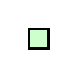
\begin{tikzpicture}[scale=0.25]\draw[thick,fill=green!20] (0,0) rectangle (1,1);\end{tikzpicture}\,); this is
followed by a linear path \textswab{L} which is satisfied probabilistically, first using accelerating techniques such as neutral bits (\,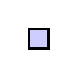
\begin{tikzpicture}[scale=0.25]\draw[thick,fill=blue!20] (0,0) rectangle (1,1);\end{tikzpicture}\,),
and then purely randomly (\,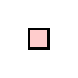
\begin{tikzpicture}[scale=0.25]\draw[thick,fill=red!20] (0,0) rectangle (1,1);\end{tikzpicture}\,). This results in a state difference $\diff\state$ which is passed to a second block. This block
uses a different non-linear path \textswab{NL~2} to connect to the negated linear path \textswab{-L} that is obtained by using an oppositely signed message difference $-\diff\expmess$; following this second path leads to
a collision.

\begin{figure}[!htb]
\begin{centering}
\def\mystrutNL{\vrule height 1.5em depth 1em width 0pt}%
\def\mystrutLin{\vrule height 2.5em depth 2em width 0pt}%

\begin{tikzpicture}[
	scale=1.2,
	transform shape,
	node distance=3em and 0em,
]
    \tikzstyle{F} = [
    		draw,
		rectangle split,
		rectangle split horizontal=false, 
		rectangle split parts=3,
		rectangle split draw splits=false, 
		rectangle split part fill={green!20, blue!20, red!20},
		text centered,
		text width=4em,
		minimum width=4em,
		minimum height=12em,
	]
	
	%%
	%% First characteristic
	%%
	\node[F] (c1) {\mystrutNL $NL~1$ \nodepart{two} \nodepart{three}\mystrutLin {\Large$L$}};
	\draw[dashed] (c1.text split west) -- (c1.text split east);
    \draw[dashed] (c1.two split west) -- (c1.two split east);
	\node[MODADD,scale=1.5,below = 2em of c1] (add1) {};
	\node[above = of c1.north, xshift=-1em] (in11) {};
	\node[above = of c1.north, xshift=1em] (in12) {$\diff\expmess$};

	\draw[line] let \p1=(in11.south),\p2=(c1.north) in (\x1,\y1) -- (\x1,\y2);
	\draw[line] let \p1=(in12.south),\p2=(c1.north) in (\x1,\y1) -- (\x1,\y2);
	\draw[line] (c1) -- node[right] {$\diff\state$} (add1);

	\draw[line] let \p1=(in11),\p2=(c1.north),\p3=(add1) in 
		(\x1,\y2+1.5em) 
		-- node[above left]{$0$} (\x3-3em,\y2+1.5em) 
		-- (\x3-3em,\y3) 
		-- node[below] {} (add1);
	
	%%
	%% Second characteristic
	%%
	\node[F, right = 8em of c1] (c2) {\mystrutNL $NL~2$\nodepart{two} \nodepart{three} \mystrutLin {\Large$-L$}};
	\draw[dashed] (c2.text split west) -- (c2.text split east);
    \draw[dashed] (c2.two split west) -- (c2.two split east);
	\node[MODADD,scale=1.5,below = 2em of c2] (add2) {};
	\node[below = of add2] (out) {};
	\node[above = of c2.north, xshift=-1em] (in21) {};
	\node[above = of c2.north, xshift=1em] (in22) {$-\diff\expmess$};

	\draw[line] (c2) -- node[right] {$-\diff\state$} (add2);
	\draw[line] let \p1=(in22.south),\p2=(c2.north) in (\x1,\y1) -- (\x1,\y2);
	\draw[line] (add2) -- (out) node[below] {0};

	\coordinate (M12) at ($(add1)!0.5!(add2)$);

	\draw[line] let \p1=(c2.north),\p2=(add1),\p3=(in21),\p4=(M12) in 
		(\x2,\y2) 
		-- (\x2,\y2-2em) 
		-- (\x4-1.5em,\y4-2em)
		-- (\x4-1.5em,\y3)
		-- (\x3,\y3)
		-- (\x3,\y1);

	\draw[line] let \p1=(in21),\p2=(c2.north),\p3=(add2) in 
		(\x1,\y2+1.5em) 
		-- node[above left]{$\diff\state$} (\x3-3em,\y2+1.5em) 
		-- (\x3-3em,\y3) 
		-- node[below] {$\diff\state$} (add2);

\end{tikzpicture}

\caption[The structure of a two-block collision attack for \sha.]{The structure of a two-block collision attack for \sha. Figure adapted from~\cite{TiKZ:Cryptographers}\label{fig:two_blocks}}
\end{centering}
\end{figure}

\medskip

The main difficulty in using non-linear paths is to find the paths themselves, as there is a large number of possible behaviours to take into account.
The search was initially done by hand for the first attack on \shaone, but automated tools were later developed to make this process much
more efficient. One can for instance cite the work of De~Cannière and Rechberger~\cite{DBLP:conf/asiacrypt/CanniereR06}, who used a guess-and-determine
approach to find new non-linear paths, leading in particular to an explicit two-block collision for \shaone reduced to the at-the-time record number of 64 steps.

The idea of the guess-and-determine method is to define a set of \emph{constraints} that encode a differential path, along with an efficient constraint-propagation
algorithm. One then starts from an underdefined initial path with many unconstrained differences (but with the conditions for the \iv and for the connecting
linear path already set) and iteratively chooses an unconstrained difference at random, assigns it a value, and propagates the consequences of this choice.
A backtracking strategy is also used to escape situations where no more valid choices are possible. A path is found when every constraint is either a signed
difference or a (possibly signed) equality.

One can also mention the alternative ``meet-in-the-middle'' approach for the construction of these paths, which was used by Yajima \etal~\cite{DBLP:conf/acisp/YajimaSNISKO07},
and later Stevens~\cite{phdstevens}. This method works by defining two partial differential paths, one expanded forward (\eg starting from the \iv) and one expanded backward
(\eg starting from the purely linear part of the path), that are then connected on a few consecutive steps.

The advantages of an automatic search of the non-linear part of the differential path over a manual one are twofold: (1) It is much faster to create new
attack instances, which allows for example to experiment quickly with several \dvs. This is particularly useful if one wants both to mount
attacks for the full function (even without running the attack completely) and attacks for a high number of reduced steps, the best \dvs in each case
being likely different. (2) The ability to generate many non-linear paths allows to search for ones that have few constraints (for instance leading
to more available neutral bits) or that can incorporate more preset constraints (that may for instance aid in the use of boomerang neutral bits).

% advantage is twofold: faster to mount new attacks, to experiment with several dvs; may lead to better paths or paths satisfying predefined constraints

% Imposes L behaviour; (no zero in five back, consecutive IFs (although also partly resolved at EUROCRYPT))
%NL A major idea of Wang \etal in their attack
%allows efficient instantiations of two blocks)
% and moar dvs too (can be dense in beginning of first round)
% also message mod, but bof, NB's fine too


\subsubsection{Classes of disturbance vectors for \shaone}
\label{sec:sha1_dvs}

We recall from \autoref{sec:dv_sha0} that the search for disturbance vectors for \shazero naturally reduces to a search among only $2^{16}$ candidates. Once a cost function
is chosen, it is simple to evaluate it on every potential \dv and one just needs to keep the best of them. Unfortunately, the message expansion of \shaone can no longer be seen as
thirty-two smaller independent message expansions, making the search space for potential \dvs significantly larger.

In the original attack from Wang \etal, the \dv was found when searching through a reduced space of size $2^{38}$, using the Hamming weight of the resulting \dvs
as the primary cost function.
Subsequently, a significant amount of work focused on finding alternate disturbance vectors in the hope of decreasing the cost of the
probabilistic phase of the attack. Manuel then noticed that all \dvs suggested in the literature could actually be concisely described by two simple classes which
lead to the best known vectors~\cite{DBLP:journals/dcc/Manuel11}; we now summarize these results.

\medskip

We start by defining an \emph{extended expanded message} for \shaone as follows:
\begin{defi}[Extended expanded message]
\label{def:eem}
Let  $\mess$  be a \shaone message block made of sixteen 32-bit message words $\mess_0, \ldots, \mess_{15}$. The \emph{extended expanded message} $\eem$ for $\mess$
is made of 144 32-bit words $\eem_{-64}, \ldots, \eem_{79}$ defined by:
\begin{equation}
\label{eq:ext_exp_mess}
\eem_i=
\left\{
\begin{array}{ll}
\mess_i, & \textnormal{ for } 0\leq i\leq 15 \\
(\eem_{i-3} \oplus \eem_{i-8} \oplus \eem_{i-14} \oplus \eem_{i-16}) \circlearrowleft 1, & \textnormal{ for } 16\leq i\leq 79\\
\eem_{i} = (\eem_{i+16} \circlearrowright 1) \oplus \eem_{i+13} \oplus \eem_{i+8} \oplus \eem_{i+2}, & \textnormal{for} -64\leq i\leq -1
\end{array}.
\right.
\end{equation}
\end{defi}
In other words, an extended expanded message expands an initial message both forwards (using \autoref{eq:exp_mess}) by 64 words, but also
backwards (using \autoref{eq:exp_mess_inv}) by a similar amount. By definition, every consecutive 80 words $\eem_i, \ldots, \eem_{i+79}$, $i \in [-64, \ldots, 0]$
of $\eem$ form a valid expanded message ``$(\eem_i)$'' for \shaone. Furthermore, it is easy to check that these 65 expanded messages are exactly the 65 possible such messages
for which sixteen consecutive words are equal to $\mess$.

We also note the following fact:
\begin{fact}[The message expansion of \shaone is a quasi-cyclic code]
If $\expmess = \expmess_0, \ldots,\linebreak \expmess_{79}$ is a valid expanded message for \shaone, then for every $i \in [0, 31]$, $\expmess^{\circlearrowleft i} \defas
\expmess_0^{\circlearrowleft i}, \ldots,\linebreak \expmess_{79}^{\circlearrowleft i}$ is a valid expanded message for \shaone.
\end{fact}
This fact, together with the notion of extended expanded message allows to define equivalence classes for expanded messages:
\begin{defi}[Equivalence class for \shaone expanded messages~\cite{DBLP:journals/dcc/Manuel11}]
Two\linebreak \shaone expanded messages $\expmess$ and $\expmess'$ are equivalent if there are two pairs $(i,j)$, $(i',j')$ in $[-64, 0] \times [0, 31]$
and an extended expanded message $\eem$ such that $\expmess = (\eem_i)^{\circlearrowleft j}$ and $\expmess' = (\eem_{i'})^{\circlearrowleft j'}$.
\end{defi}
In other words, two expanded messages are equivalent if they can be generated from the same, possibly rotated, extended expanded message. It should be noted
however that a message necessarily belongs to many distinct such equivalence classes.

As the disturbance vectors are expanded messages themselves, one can then use equivalence classes as a natural way to segment the search space for good \dvs. For instance,
Manuel searched for candidates among all classes of extended expanded messages defined from windows of Hamming weight up to four, and for some classes defined by
windows of weight five and six. It followed from this search that all good \dvs, including all the ones described in previous work, come from two equivalence classes.
The 16-word messages generating the extended expanded messages of the two classes (up to rotation) are shown in \autoref{fig:dv_types}\footnote{The messages in this
figure are given using an unsigned difference notation. In \autoref{def:eem}, we gave the definition using a ``normal'' message $\in \{\{0,1\}^{32}\}^{16}$. As
a disturbance vector is eventually used to define the difference between two messages, we think that using such a notation is appropriate in this case.}.

\begin{figure}[!ht]
\begin{center}
\begin{tabular}{cc}
\nodiff \nodiff \nodiff \nodiff \nodiff \nodiff \nodiff \nodiff \nodiff \nodiff \nodiff \nodiff \nodiff \nodiff
\nodiff \nodiff \nodiff \nodiff \nodiff \nodiff \nodiff \nodiff \nodiff \nodiff \nodiff \nodiff \nodiff \nodiff \nodiff \nodiff \nodiff \nodiff&
\nodiff \nodiff \nodiff \nodiff \nodiff \nodiff \nodiff \nodiff \nodiff \nodiff \nodiff \nodiff \nodiff \nodiff
\nodiff \nodiff \nodiff \nodiff \nodiff \nodiff \nodiff \nodiff \nodiff \nodiff \nodiff \nodiff \nodiff \nodiff \nodiff \nodiff \nodiff \nodiff \\
\nodiff \nodiff \nodiff \nodiff \nodiff \nodiff \nodiff \nodiff \nodiff \nodiff \nodiff \nodiff \nodiff \nodiff
\nodiff \nodiff \nodiff \nodiff \nodiff \nodiff \nodiff \nodiff \nodiff \nodiff \nodiff \nodiff \nodiff \nodiff \nodiff \nodiff \nodiff \nodiff&
\onediff \nodiff \nodiff \nodiff \nodiff \nodiff \nodiff \nodiff \nodiff \nodiff \nodiff \nodiff \nodiff \nodiff
\nodiff \nodiff \nodiff \nodiff \nodiff \nodiff \nodiff \nodiff \nodiff \nodiff \nodiff \nodiff \nodiff \nodiff \nodiff \nodiff \nodiff \nodiff \\
\nodiff \nodiff \nodiff \nodiff \nodiff \nodiff \nodiff \nodiff \nodiff \nodiff \nodiff \nodiff \nodiff \nodiff
\nodiff \nodiff \nodiff \nodiff \nodiff \nodiff \nodiff \nodiff \nodiff \nodiff \nodiff \nodiff \nodiff \nodiff \nodiff \nodiff \nodiff \nodiff&
\nodiff \nodiff \nodiff \nodiff \nodiff \nodiff \nodiff \nodiff \nodiff \nodiff \nodiff \nodiff \nodiff \nodiff
\nodiff \nodiff \nodiff \nodiff \nodiff \nodiff \nodiff \nodiff \nodiff \nodiff \nodiff \nodiff \nodiff \nodiff \nodiff \nodiff \nodiff \nodiff \\
\nodiff \nodiff \nodiff \nodiff \nodiff \nodiff \nodiff \nodiff \nodiff \nodiff \nodiff \nodiff \nodiff \nodiff
\nodiff \nodiff \nodiff \nodiff \nodiff \nodiff \nodiff \nodiff \nodiff \nodiff \nodiff \nodiff \nodiff \nodiff \nodiff \nodiff \nodiff \nodiff&
\onediff \nodiff \nodiff \nodiff \nodiff \nodiff \nodiff \nodiff \nodiff \nodiff \nodiff \nodiff \nodiff \nodiff
\nodiff \nodiff \nodiff \nodiff \nodiff \nodiff \nodiff \nodiff \nodiff \nodiff \nodiff \nodiff \nodiff \nodiff \nodiff \nodiff \nodiff \nodiff \\
\nodiff \nodiff \nodiff \nodiff \nodiff \nodiff \nodiff \nodiff \nodiff \nodiff \nodiff \nodiff \nodiff \nodiff
\nodiff \nodiff \nodiff \nodiff \nodiff \nodiff \nodiff \nodiff \nodiff \nodiff \nodiff \nodiff \nodiff \nodiff \nodiff \nodiff \nodiff \nodiff&
\nodiff \nodiff \nodiff \nodiff \nodiff \nodiff \nodiff \nodiff \nodiff \nodiff \nodiff \nodiff \nodiff \nodiff
\nodiff \nodiff \nodiff \nodiff \nodiff \nodiff \nodiff \nodiff \nodiff \nodiff \nodiff \nodiff \nodiff \nodiff \nodiff \nodiff \nodiff \nodiff \\
\nodiff \nodiff \nodiff \nodiff \nodiff \nodiff \nodiff \nodiff \nodiff \nodiff \nodiff \nodiff \nodiff \nodiff
\nodiff \nodiff \nodiff \nodiff \nodiff \nodiff \nodiff \nodiff \nodiff \nodiff \nodiff \nodiff \nodiff \nodiff \nodiff \nodiff \nodiff \nodiff&
\nodiff \nodiff \nodiff \nodiff \nodiff \nodiff \nodiff \nodiff \nodiff \nodiff \nodiff \nodiff \nodiff \nodiff
\nodiff \nodiff \nodiff \nodiff \nodiff \nodiff \nodiff \nodiff \nodiff \nodiff \nodiff \nodiff \nodiff \nodiff \nodiff \nodiff \nodiff \nodiff \\
\nodiff \nodiff \nodiff \nodiff \nodiff \nodiff \nodiff \nodiff \nodiff \nodiff \nodiff \nodiff \nodiff \nodiff
\nodiff \nodiff \nodiff \nodiff \nodiff \nodiff \nodiff \nodiff \nodiff \nodiff \nodiff \nodiff \nodiff \nodiff \nodiff \nodiff \nodiff \nodiff&
\nodiff \nodiff \nodiff \nodiff \nodiff \nodiff \nodiff \nodiff \nodiff \nodiff \nodiff \nodiff \nodiff \nodiff
\nodiff \nodiff \nodiff \nodiff \nodiff \nodiff \nodiff \nodiff \nodiff \nodiff \nodiff \nodiff \nodiff \nodiff \nodiff \nodiff \nodiff \nodiff \\
\nodiff \nodiff \nodiff \nodiff \nodiff \nodiff \nodiff \nodiff \nodiff \nodiff \nodiff \nodiff \nodiff \nodiff
\nodiff \nodiff \nodiff \nodiff \nodiff \nodiff \nodiff \nodiff \nodiff \nodiff \nodiff \nodiff \nodiff \nodiff \nodiff \nodiff \nodiff \nodiff&
\nodiff \nodiff \nodiff \nodiff \nodiff \nodiff \nodiff \nodiff \nodiff \nodiff \nodiff \nodiff \nodiff \nodiff
\nodiff \nodiff \nodiff \nodiff \nodiff \nodiff \nodiff \nodiff \nodiff \nodiff \nodiff \nodiff \nodiff \nodiff \nodiff \nodiff \nodiff \nodiff \\
\nodiff \nodiff \nodiff \nodiff \nodiff \nodiff \nodiff \nodiff \nodiff \nodiff \nodiff \nodiff \nodiff \nodiff
\nodiff \nodiff \nodiff \nodiff \nodiff \nodiff \nodiff \nodiff \nodiff \nodiff \nodiff \nodiff \nodiff \nodiff \nodiff \nodiff \nodiff \nodiff&
\nodiff \nodiff \nodiff \nodiff \nodiff \nodiff \nodiff \nodiff \nodiff \nodiff \nodiff \nodiff \nodiff \nodiff
\nodiff \nodiff \nodiff \nodiff \nodiff \nodiff \nodiff \nodiff \nodiff \nodiff \nodiff \nodiff \nodiff \nodiff \nodiff \nodiff \nodiff \nodiff \\
\nodiff \nodiff \nodiff \nodiff \nodiff \nodiff \nodiff \nodiff \nodiff \nodiff \nodiff \nodiff \nodiff \nodiff
\nodiff \nodiff \nodiff \nodiff \nodiff \nodiff \nodiff \nodiff \nodiff \nodiff \nodiff \nodiff \nodiff \nodiff \nodiff \nodiff \nodiff \nodiff&
\nodiff \nodiff \nodiff \nodiff \nodiff \nodiff \nodiff \nodiff \nodiff \nodiff \nodiff \nodiff \nodiff \nodiff
\nodiff \nodiff \nodiff \nodiff \nodiff \nodiff \nodiff \nodiff \nodiff \nodiff \nodiff \nodiff \nodiff \nodiff \nodiff \nodiff \nodiff \nodiff \\
\nodiff \nodiff \nodiff \nodiff \nodiff \nodiff \nodiff \nodiff \nodiff \nodiff \nodiff \nodiff \nodiff \nodiff
\nodiff \nodiff \nodiff \nodiff \nodiff \nodiff \nodiff \nodiff \nodiff \nodiff \nodiff \nodiff \nodiff \nodiff \nodiff \nodiff \nodiff \nodiff&
\nodiff \nodiff \nodiff \nodiff \nodiff \nodiff \nodiff \nodiff \nodiff \nodiff \nodiff \nodiff \nodiff \nodiff
\nodiff \nodiff \nodiff \nodiff \nodiff \nodiff \nodiff \nodiff \nodiff \nodiff \nodiff \nodiff \nodiff \nodiff \nodiff \nodiff \nodiff \nodiff \\
\nodiff \nodiff \nodiff \nodiff \nodiff \nodiff \nodiff \nodiff \nodiff \nodiff \nodiff \nodiff \nodiff \nodiff
\nodiff \nodiff \nodiff \nodiff \nodiff \nodiff \nodiff \nodiff \nodiff \nodiff \nodiff \nodiff \nodiff \nodiff \nodiff \nodiff \nodiff \nodiff&
\nodiff \nodiff \nodiff \nodiff \nodiff \nodiff \nodiff \nodiff \nodiff \nodiff \nodiff \nodiff \nodiff \nodiff
\nodiff \nodiff \nodiff \nodiff \nodiff \nodiff \nodiff \nodiff \nodiff \nodiff \nodiff \nodiff \nodiff \nodiff \nodiff \nodiff \nodiff \nodiff \\
\nodiff \nodiff \nodiff \nodiff \nodiff \nodiff \nodiff \nodiff \nodiff \nodiff \nodiff \nodiff \nodiff \nodiff
\nodiff \nodiff \nodiff \nodiff \nodiff \nodiff \nodiff \nodiff \nodiff \nodiff \nodiff \nodiff \nodiff \nodiff \nodiff \nodiff \nodiff \nodiff&
\nodiff \nodiff \nodiff \nodiff \nodiff \nodiff \nodiff \nodiff \nodiff \nodiff \nodiff \nodiff \nodiff \nodiff
\nodiff \nodiff \nodiff \nodiff \nodiff \nodiff \nodiff \nodiff \nodiff \nodiff \nodiff \nodiff \nodiff \nodiff \nodiff \nodiff \nodiff \nodiff \\
\nodiff \nodiff \nodiff \nodiff \nodiff \nodiff \nodiff \nodiff \nodiff \nodiff \nodiff \nodiff \nodiff \nodiff
\nodiff \nodiff \nodiff \nodiff \nodiff \nodiff \nodiff \nodiff \nodiff \nodiff \nodiff \nodiff \nodiff \nodiff \nodiff \nodiff \nodiff \nodiff&
\nodiff \nodiff \nodiff \nodiff \nodiff \nodiff \nodiff \nodiff \nodiff \nodiff \nodiff \nodiff \nodiff \nodiff
\nodiff \nodiff \nodiff \nodiff \nodiff \nodiff \nodiff \nodiff \nodiff \nodiff \nodiff \nodiff \nodiff \nodiff \nodiff \nodiff \nodiff \nodiff \\
\nodiff \nodiff \nodiff \nodiff \nodiff \nodiff \nodiff \nodiff \nodiff \nodiff \nodiff \nodiff \nodiff \nodiff
\nodiff \nodiff \nodiff \nodiff \nodiff \nodiff \nodiff \nodiff \nodiff \nodiff \nodiff \nodiff \nodiff \nodiff \nodiff \nodiff \nodiff \nodiff&
\nodiff \nodiff \nodiff \nodiff \nodiff \nodiff \nodiff \nodiff \nodiff \nodiff \nodiff \nodiff \nodiff \nodiff
\nodiff \nodiff \nodiff \nodiff \nodiff \nodiff \nodiff \nodiff \nodiff \nodiff \nodiff \nodiff \nodiff \nodiff \nodiff \nodiff \nodiff \nodiff \\
\nodiff \nodiff \nodiff \nodiff \nodiff \nodiff \nodiff \nodiff \nodiff \nodiff \nodiff \nodiff \nodiff \nodiff
\nodiff \nodiff \nodiff \nodiff \nodiff \nodiff \nodiff \nodiff \nodiff \nodiff \nodiff \nodiff \nodiff \nodiff \nodiff \nodiff \nodiff \onediff&
\nodiff \nodiff \nodiff \nodiff \nodiff \nodiff \nodiff \nodiff \nodiff \nodiff \nodiff \nodiff \nodiff \nodiff
\nodiff \nodiff \nodiff \nodiff \nodiff \nodiff \nodiff \nodiff \nodiff \nodiff \nodiff \nodiff \nodiff \nodiff \nodiff \nodiff \nodiff \onediff \\
\end{tabular}
\end{center}
\caption[Type I and type II disturbance vectors.]{The messages defining the class of type I (left) and type II (right) disturbance vectors, given as sixteen 32-bit words $\mess_0, \ldots, \mess_{15}$,
with $\mess_0$ on top.\label{fig:dv_types}}
\end{figure}

\noindent
Following this observation, Manuel termed I$(i,j)$ and II$(i,j)$ the disturbance vectors $(\eem_{-i})^{\circlearrowleft j}$ where
$\eem$ is generated from the messages of type I and II of \autoref{fig:dv_types} respectively.

\subsubsection{Exact cost functions for disturbance vectors}
%\subsubsection{Exact probability of chains of local collisions}
\label{sec:chain_lc}

We have already mentioned the role played by the cost functions when choosing a disturbance vector, both in the case of \shazero in \autoref{sec:dv_sha0} and in the case
of \shaone in the previous \autoref{sec:sha1_dvs}. A first basic such function is simply to take the Hamming weight of a vector (\ie to count the number of local collisions)
over the steps where we expect the attack to be purely probabilistic (\eg starting from step 20). Even in the case of \shazero, we have seen that some additional interactions between
local collisions need to be taken into account to make this function more accurate. The same sort of interactions is also present in the case of \shaone, and some new ones may appear as well, especially
because several local collisions may now be started on the same step.

\medskip

\paragraph{Bit compression}
$\phantom{bouh}$

\medskip

\noindent
A first new kind of interaction between local collisions that is favourable to the cryptanalyst is the effect used in the technique of \emph{bit compression} introduced by Wang \etal \cite{DBLP:conf/crypto/WangYY05a}
as a \emph{special counting rule} and later named as such by Yajima \etal~\cite{DBLP:conf/ccs/YajimaINSSKO08}. Under certain conditions, this technique allows to significantly
improve the joint probability of two (or more) neighbouring local collisions being successful by making it as high as for a single one. In a nutshell, the idea is to introduce the initial perturbations
using a chain of differences all
having the same sign, except for the last one, and to let the carry propagate from the first
perturbation to the other ones instead of preventing such a propagation every time.
Let us see how this may work on an example with three neighbouring differences.

\begin{example}[Compression of three differences]
\label{ex:bit_comp}
Consider a chain of differences of the form $\ldots\mnodiff\monediffu\monediffd\monediffd\mnodiff\ldots$ added to a state with no difference $\ldots\mnodiff\mnodiff\mnodiff\mnodiff\mnodiff\ldots$.
It is most useful in this case to first consider the differences as modular ones. If we call $x,\widetilde{x}$ and $y,\widetilde{y}$ the two states that are added together, we
have $\widetilde{x} = x - 2^{i} - 2^{i+1} + 2^{i+2}$ for some value $i$. Now we want to determine what are the probabilities of some of the possible resulting XOR differences between $x + y$ and $\widetilde{x} + \widetilde{y}$.

Using a traditional view and treating all differences separately (which is what would happen if these were perturbations of local collisions seen independently), we would like to have no
carry propagation at any of the three position, to obtain an XOR difference on the same three positions where differences were introduced. It is easy to see that this imposes three conditions
on $x + y$, as it means that we want $\widetilde{x} + \widetilde{y} = (x + y) \oplus 2^{i} \oplus 2^{i+1} \oplus 2^{i+2}$, which translates to bits $i$, $i+1$ and $i+2$ of $x+y$ being 1, 1 and 0 respectively.
The probability of this happening is thus $2^{-3}$.

However, as we have $2^{i+2} - 2^{i+1} - 2^{i} = 2^{i}$, the alternative XOR difference $\widetilde{x} + \widetilde{y} = (x + y) \oplus 2^{i}$ only imposes one condition on $x + y$, namely that bit $i$
must be 0; this difference may then happen with probability $2^{-1}$.
\end{example}

We can use the effect showed in \autoref{ex:bit_comp} to increase the probability of a successful introduction of perturbations in series of local collisions; this is however at the condition that
the ``compressed'' XOR difference obtained as a result is compatible with the following corrections, which are still located on multiple bits. Fortunately, this condition is always fulfilled
provided: (1) That the single difference is not absorbed or flipped in a Boolean function (this is the usual condition for a successful correction); (2) That the chain of consecutive differences
is not broken through the bit rotations (this is a ``hard'' condition that determines if a series of neighbouring local collisions can indeed be compressed). We illustrate this by continuing
our previous example.

\begin{example}[Correction of compressed differences]
\label{ex:bit_comp2}
Let us use modular differences again. Consider the case of \autoref{ex:bit_comp} and assume that the introduction of the perturbation resulted in the modular and XOR difference
$\widetilde{x} + \widetilde{y} = (x + y) + 2^{i}  = (x + y) \oplus 2^{i}$. Assume that this difference is preserved through the step function, excluding the addition of the message,
resulting in a partial state $z, \widetilde{z}$ with $\widetilde{z} = z + 2^{i}$. This partial state is rotated to the left by $r \in \{0, 5, 30\}$ in the computation of the new state,
and the differences in the message at this point are at positions $\alpha = i + r\mod32$, $\beta = i+1+r \mod 32$, $\gamma = i+2+r \mod 32$ and of sign opposite the ones of the initial perturbation,
\ie we have $m, \widetilde{m}$ with $\widetilde{m} = m + 2^{\alpha} + 2^{\beta} - 2^{\gamma}$. If $\alpha < \beta < \gamma$, we then have $\widetilde{m} = m - 2^{\alpha}$. In that case,
$(\widetilde{z} \circlearrowleft r) + \widetilde{m}$ = $(z \circlearrowleft r) + 2^{\alpha} + m - 2^{\alpha}$ = $(z \circlearrowleft r) + m$, and the correction is indeed successful.
\end{example}

It is worth noting that because only a single state difference needs to be preserved through the Boolean functions during the correction, the probability of all corrections of compressed
local collisions being successful is also much higher, compared to the uncompressed case.

To summarize, local collisions starting at the same step and at neighbouring bit positions that remain consecutive through left rotations by 5 and 30 (\ie the considered bit positions
do not include bit 1 or 26 and bits to their left) can be compressed by choosing a proper signing for the initial perturbation. The probability of the resulting compressed collision
to be successful is the same as the success probability of a single local collision.

Finally, let us note that compressing local collisions does not actually hinder in any way their
chance of being successful in the ``traditional'' (independent) way. For instance, two local collisions in no particular position during an XOR round have a ``theoretical'' joint success probability of
$2^{-8}$ when considered independent and of $2^{-4}$ if they are compressed (as per \autoref{sec:diffs_ana}). The two successful events being independent, the total theoretical success probability of these collisions is thence $2^{-3.91}$.
It may thus appear that compressed local collisions actually have a \emph{higher} probability than single ones. This is actually not the case, as we explain next.

\paragraph{Bit decompression}
$\phantom{bouh}$

\medskip

\noindent
We now use the insight gained from the analysis of the bit compression technique to come closer to computing the exact success probability of local collisions.
The observation we make here is that in the same way as neighbouring XOR bit differences of appropriate sign can be compressed into a single modular difference, a single XOR difference
can be ``decompressed'' into a series of multiple modular ones. Similarly as for bit compression, if this difference is the perturbation of a local collision, the corrections may still be effective
if they can themselves be decompressed.

In other words, it is not necessary that the introduction of the perturbation of a local collision does not trigger a difference in carry propagations; even if this is the case, the local
collision may still be successful if the resulting state difference is preserved by the Boolean functions (and if the carry chain is not broken by rotations during the corrections). Thus, the success probability of
a single local collision not on a rotation boundary is strictly higher than the probability obtained from the analysis of \autoref{sec:diffs_ana} (as it is).

We may rephrase this in a slightly more formal way as follows:

\medskip

Consider a local collision started by an initial perturbation on $m_s$ and $\widetilde{m_s}$ of positive sign at position $i < 31$, \ie with a signed bit difference $\ldots\mnodiff\monediffu\mnodiff\ldots$.
This corresponds to a modular difference $\widetilde{m_s} = m_s + 2^i$. Call $x$, $\widetilde{x}$ and $y$, $\widetilde{y}$ the state to which the message $m_s$, $\widetilde{m_s}$ is added and the result of this addition
respectively. The probability (over the values of $x$) of having a signed difference $\ldots\mnodiff\monediffu\mnodiff\ldots$ for $y$, $\widetilde{y}$ is $2^{-1}$.
However, we also have $\widetilde{m_s} = m_s - \sum_{j = i}^{k - 1}2^j + 2^k$ for any $k < 32$. Thus we can write $\widetilde{y} = \widetilde{x} + \widetilde{m_s} = x + m_s - \sum_{j = i}^{k - 1}2^j + 2^k$. The
probability of having a difference $\ldots\mnodiff\monediffu\monediffd\mnodiff\ldots$ between $\widetilde{y}$ and $y$ is thus $2^{-2}$; more generally, the probability of
having a difference $\ldots\mnodiff\monediffu\underbrace{\monediffd\ldots\monediffd}_{u~\text{times}}\mnodiff\ldots$ between $\widetilde{y}$ and $y$ (with $i+u+1 < 32$) is $2^{-u-1}$.

For an initial difference of weight $u+1$, the corrections on subsequent message words $m_{s+o}$, $\widetilde{m_{s+o}}$ are of the form $\widetilde{m_{s+o}} = m_{s+o} - 2^{i+r\mod 32}$, $r \in \{0,5,30\}$.
An initial perturbation that resulted in a difference on $y$, $\widetilde{y}$ of weight $u+1$ can thus be corrected at every step only if $i+r\mod 32 \leq i+u+r\mod 32$, because the equality
$\widetilde{m_{s+o}} = m_{s+o} + \sum_{j = i+r \mod 32}^{i+r+u-1 \mod 32}2^j - 2^{i+r+u \mod 32}$ must hold.

Now assume that the maximal weight of an initial perturbation that can be corrected is $v$, and that for the sake of simplicity all induced perturbations are in an XOR round in no particular position
(meaning that no correction is on the MSB), then the success probability of having a local collision is $\sum_{i=1}^{v}2^{-4v}$, which is higher than the probability $2^{-4}$ obtained by considering
only the signed difference $\ldots\mnodiff\monediffu\mnodiff\ldots$.

A complete analysis of the impact of carry propagation on the success probability of a single local collision was done
by Mendel \etal for all Boolean functions and positions of the perturbation~\cite{DBLP:conf/fse/MendelPRR06a}. Manuel also performed experiments validating this analysis~\cite{DBLP:journals/dcc/Manuel11}
(in particular, these results seem to show that for a single local collision, no additional effect contributes to the success probability).

\medskip

To conclude this part and the previous one, we have seen that the interaction of XOR and modular differences in \sha leads to a slight \emph{differential} effect for the disturbance vector. A single
message difference actually defines several, not mutually exclusive, local collision patterns. Even though one of these patterns is much more likely than the others (\ie the one with all possible compressions
effectively done, and no decompression), the contribution of the remaining ones is not nil.

\paragraph{Joint local collision analysis}
$\phantom{bouh}$

\medskip

\noindent
We have just considered how the propagation of carries may influence the probability of a single local collision and of neighbouring local collisions started on the same step. We now consider how to account for similar effects
that impact the joint success probability of local collisions sharing some common steps. We have already mentioned in \autoref{sec:dv_sha0} that an analysis in the spirit of \autoref{sec:diffs_ana} may be done
on closely interacting local collisions (for instance on local collisions that share some correction bits or that have some corrections interacting together through the Boolean functions).
However, this does not take into account the effects of carries, and a more precise study is thus
possible.

We now summarize the \emph{joint local collision analysis} (JLCA) approach of Stevens \cite{phdstevens,DBLP:conf/eurocrypt/Stevens13}, which allows to compute the exact best probability of a disturbance vector
by considering all interactions between non-disjoint local collisions. This results in a very good ``exact'' cost function for \dvs of \shaone.

\medskip

The objective here is actually slightly more generic: for a given \dv, there is some liberty in the choice of the actual message differences (\eg by specifying their sign), and we have already seen that this
may impact the success probability of local collisions. These variations should be taken into account when comparing \dvs together, and only the message differences resulting in the best probability should
be considered. Going further, for a given range of steps, we may want to determine which initial and final state differences yield the best probability.
Thus we may reformulate our objective as wanting to find the maximum success probability for a given \dv and a prescribed number of steps over the choice of compatible signed message differences and initial
and final state differences.

To fulfill this objective, we may simply try (for a given configuration) to enumerate all differential paths and sum their probabilities. However, although this was feasible for a single local collision
(cf. \cite{DBLP:conf/fse/MendelPRR06a}),
the amount of paths to consider makes this task computationally intractable in general. The idea of Stevens to get around this limitation is to use a notion of \emph{reduced} paths together with
(equivalence) classes of message differences. A reduced path is essentially obtained from its non-reduced analogue by removing differences not interacting with the initial and final differences. Such
paths can easily be enumerated, and most importantly it is possible to compute their associated ``cumulative probabilities'' which is (for a given reduced path and a given message difference) the sum of
the probabilities of all possible complements to the reduced path that result in a valid overall path. Although the number of possible message differences to consider may be big, Stevens also shows how
to find equivalence classes yielding the same probability for all their members. It is then enough to perform the computation for one representative of every class.

%This is essentially an exhaustive analysis taking into account all local collisions together, using which one can determine the highest possible success probability.
%This analysis also produces a minimal set of sufficient conditions which, when all fulfilled, ensure that a pair of messages follows the linear path;
%the conditions are minimal in the sense that meeting all of them happens with the highest probability that was computed by the analysis.
%Although a direct approach is clearly unfeasible (as it would require dealing with an exponentially growing amount of possible differential paths),
%JLCA can be done practically by exploiting the large amount of redundancy between all the differential paths to a very large extent.

\medskip

The above strategy allows to exactly compute the best achievable probability for a given \dv over a given range of steps. However, one should keep in mind that the \dv with the best such
probability (for the range of steps one wishes to consider) is not necessarily the one most suited to an attack. Indeed, somehow in the same way as \dvs were disqualified in the original \shazero
attacks because of incompatibilities in the IF round (for the model used at the time), a \dv with high associated probability may be a worse choice than another with a lower probability if the former
makes it harder to find a good non-linear part for the first round than the latter, or similarly if it makes it harder to use accelerating techniques.

These last criteria are much harder to capture into a cost function, and there were no attempts to do so in the literature. Ultimately, the complexity of the beginning of an attack can only
be precisely determined by evaluating the speed at which an efficient implementation produces partial solutions up to a step where no freedom remains.
The cost functions as presented in this entire section are then a very useful tool to precisely extrapolate the complexity of a full attack from this point on.
